\documentclass[ignorenonframetext,]{beamer}
\setbeamertemplate{caption}[numbered]
\setbeamertemplate{caption label separator}{: }
\setbeamercolor{caption name}{fg=normal text.fg}
\beamertemplatenavigationsymbolsempty
\usepackage{lmodern}
\usepackage{amssymb,amsmath}
\usepackage{ifxetex,ifluatex}
\usepackage{fixltx2e} % provides \textsubscript
\ifnum 0\ifxetex 1\fi\ifluatex 1\fi=0 % if pdftex
\usepackage[T1]{fontenc}
\usepackage[utf8]{inputenc}
\else % if luatex or xelatex
\ifxetex
\usepackage{mathspec}
\else
\usepackage{fontspec}
\fi
\defaultfontfeatures{Ligatures=TeX,Scale=MatchLowercase}
\fi
\usetheme{Warsaw}
% use upquote if available, for straight quotes in verbatim environments
\IfFileExists{upquote.sty}{\usepackage{upquote}}{}
% use microtype if available
\IfFileExists{microtype.sty}{%
\usepackage{microtype}
\UseMicrotypeSet[protrusion]{basicmath} % disable protrusion for tt fonts
}{}
\newif\ifbibliography
\usepackage{color}
\usepackage{fancyvrb}
\newcommand{\VerbBar}{|}
\newcommand{\VERB}{\Verb[commandchars=\\\{\}]}
\DefineVerbatimEnvironment{Highlighting}{Verbatim}{commandchars=\\\{\}}
% Add ',fontsize=\small' for more characters per line
\usepackage{framed}
\definecolor{shadecolor}{RGB}{248,248,248}
\newenvironment{Shaded}{\begin{snugshade}}{\end{snugshade}}
\newcommand{\KeywordTok}[1]{\textcolor[rgb]{0.13,0.29,0.53}{\textbf{{#1}}}}
\newcommand{\DataTypeTok}[1]{\textcolor[rgb]{0.13,0.29,0.53}{{#1}}}
\newcommand{\DecValTok}[1]{\textcolor[rgb]{0.00,0.00,0.81}{{#1}}}
\newcommand{\BaseNTok}[1]{\textcolor[rgb]{0.00,0.00,0.81}{{#1}}}
\newcommand{\FloatTok}[1]{\textcolor[rgb]{0.00,0.00,0.81}{{#1}}}
\newcommand{\ConstantTok}[1]{\textcolor[rgb]{0.00,0.00,0.00}{{#1}}}
\newcommand{\CharTok}[1]{\textcolor[rgb]{0.31,0.60,0.02}{{#1}}}
\newcommand{\SpecialCharTok}[1]{\textcolor[rgb]{0.00,0.00,0.00}{{#1}}}
\newcommand{\StringTok}[1]{\textcolor[rgb]{0.31,0.60,0.02}{{#1}}}
\newcommand{\VerbatimStringTok}[1]{\textcolor[rgb]{0.31,0.60,0.02}{{#1}}}
\newcommand{\SpecialStringTok}[1]{\textcolor[rgb]{0.31,0.60,0.02}{{#1}}}
\newcommand{\ImportTok}[1]{{#1}}
\newcommand{\CommentTok}[1]{\textcolor[rgb]{0.56,0.35,0.01}{\textit{{#1}}}}
\newcommand{\DocumentationTok}[1]{\textcolor[rgb]{0.56,0.35,0.01}{\textbf{\textit{{#1}}}}}
\newcommand{\AnnotationTok}[1]{\textcolor[rgb]{0.56,0.35,0.01}{\textbf{\textit{{#1}}}}}
\newcommand{\CommentVarTok}[1]{\textcolor[rgb]{0.56,0.35,0.01}{\textbf{\textit{{#1}}}}}
\newcommand{\OtherTok}[1]{\textcolor[rgb]{0.56,0.35,0.01}{{#1}}}
\newcommand{\FunctionTok}[1]{\textcolor[rgb]{0.00,0.00,0.00}{{#1}}}
\newcommand{\VariableTok}[1]{\textcolor[rgb]{0.00,0.00,0.00}{{#1}}}
\newcommand{\ControlFlowTok}[1]{\textcolor[rgb]{0.13,0.29,0.53}{\textbf{{#1}}}}
\newcommand{\OperatorTok}[1]{\textcolor[rgb]{0.81,0.36,0.00}{\textbf{{#1}}}}
\newcommand{\BuiltInTok}[1]{{#1}}
\newcommand{\ExtensionTok}[1]{{#1}}
\newcommand{\PreprocessorTok}[1]{\textcolor[rgb]{0.56,0.35,0.01}{\textit{{#1}}}}
\newcommand{\AttributeTok}[1]{\textcolor[rgb]{0.77,0.63,0.00}{{#1}}}
\newcommand{\RegionMarkerTok}[1]{{#1}}
\newcommand{\InformationTok}[1]{\textcolor[rgb]{0.56,0.35,0.01}{\textbf{\textit{{#1}}}}}
\newcommand{\WarningTok}[1]{\textcolor[rgb]{0.56,0.35,0.01}{\textbf{\textit{{#1}}}}}
\newcommand{\AlertTok}[1]{\textcolor[rgb]{0.94,0.16,0.16}{{#1}}}
\newcommand{\ErrorTok}[1]{\textcolor[rgb]{0.64,0.00,0.00}{\textbf{{#1}}}}
\newcommand{\NormalTok}[1]{{#1}}
\usepackage{graphicx,grffile}
\makeatletter
\def\maxwidth{\ifdim\Gin@nat@width>\linewidth\linewidth\else\Gin@nat@width\fi}
\def\maxheight{\ifdim\Gin@nat@height>\textheight0.8\textheight\else\Gin@nat@height\fi}
\makeatother
% Scale images if necessary, so that they will not overflow the page
% margins by default, and it is still possible to overwrite the defaults
% using explicit options in \includegraphics[width, height, ...]{}
\setkeys{Gin}{width=\maxwidth,height=\maxheight,keepaspectratio}

% Prevent slide breaks in the middle of a paragraph:
\widowpenalties 1 10000
\raggedbottom

\AtBeginPart{
\let\insertpartnumber\relax
\let\partname\relax
\frame{\partpage}
}
\AtBeginSection{
\ifbibliography
\else
\let\insertsectionnumber\relax
\let\sectionname\relax
\frame{\sectionpage}
\fi
}
\AtBeginSubsection{
\let\insertsubsectionnumber\relax
\let\subsectionname\relax
\frame{\subsectionpage}
}

\setlength{\parindent}{0pt}
\setlength{\parskip}{6pt plus 2pt minus 1pt}
\setlength{\emergencystretch}{3em}  % prevent overfull lines
\providecommand{\tightlist}{%
\setlength{\itemsep}{0pt}\setlength{\parskip}{0pt}}
\setcounter{secnumdepth}{0}

\title{Wizualizacja danych}
\author{Piotr Guzik, Lucjan Janowski, Krzysztof Rusek}
\date{24 października 2017}

\begin{document}
\frame{\titlepage}

\begin{frame}{Po co wizualizować dane}

\begin{itemize}
\tightlist
\item
  Lepiej analizujemy obrazy niż ``suche'' liczby
\item
  Można dostrzec pewne charakterystyki problemu, z którym mamy do
  czynienia
\item
  Można zauważyć potencjalne problemy
\item
  Aby odnaleźć dane odstające (np. błędne)
\item
  Aby podzielić się wynikami analizy z innymi - jeden obraz wart więcej
  niż 1000 słów ;)
\end{itemize}

\end{frame}

\begin{frame}{Po co wizualizować dane?}

\begin{center}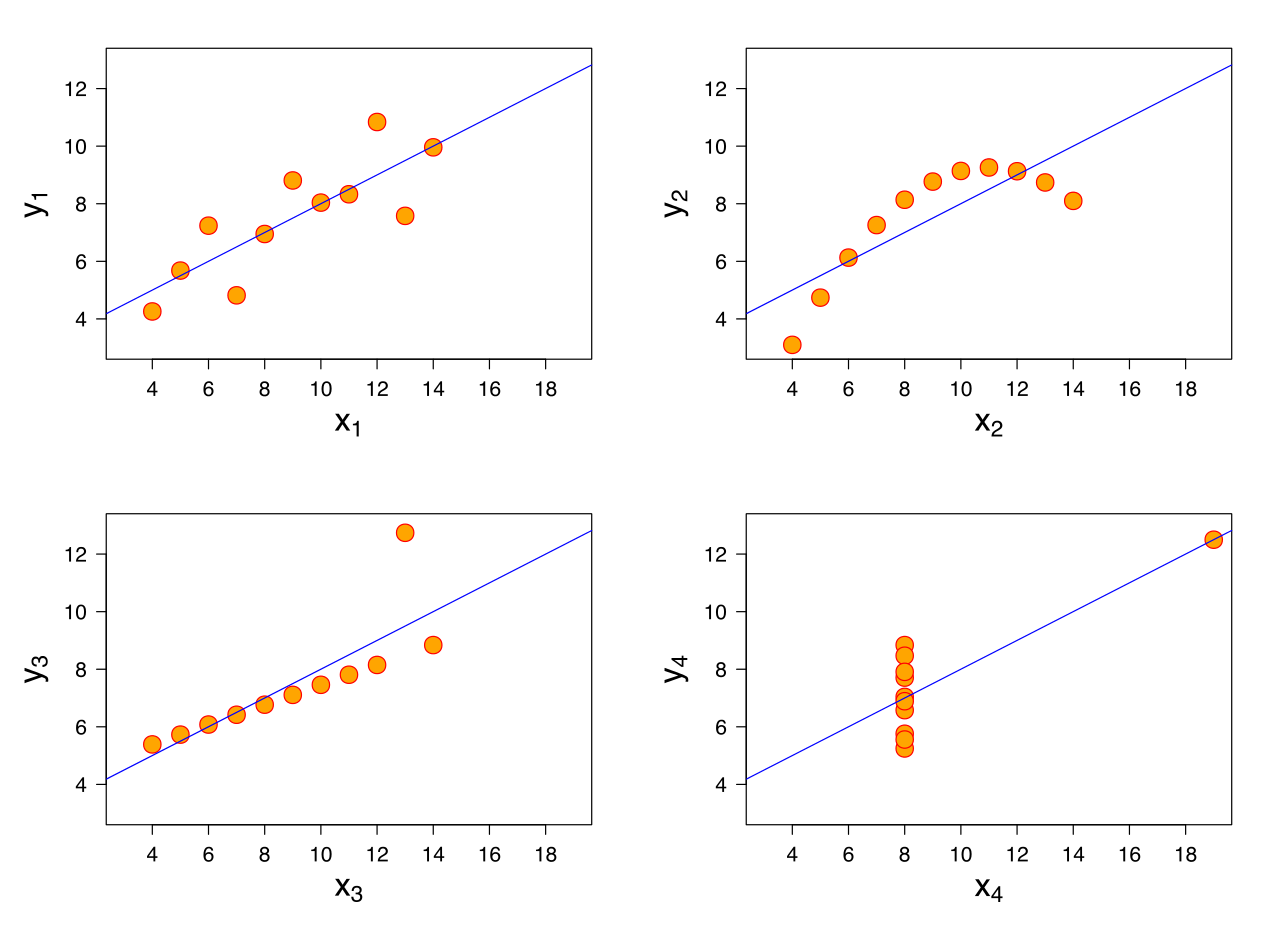
\includegraphics[width=300px]{images/kwartet} \end{center}

\end{frame}

\begin{frame}{Po co wizualizować dane?}

Na poprzednim rysunku przedstawione były 4 różne zbiory danych, które
jednak miały takie same charakterystyki:

\begin{itemize}
\tightlist
\item
  Średnia wartość zmiennej ``x'' równa 9, średnia wartość zmiennej ``y''
  równa 7.5
\item
  wariancja zmiennej ``x'' równa 11, wariancja zmiennej ``y'' równa 4.12
\item
  korelacja obydwu zmiennych równa 0.816
\item
  najlepiej dopasowany model regresji liniowej to \(y=3+0.5x\)
\end{itemize}

\end{frame}

\begin{frame}{Po co wizualizować dane?}

\includegraphics{W4_files/figure-beamer/unnamed-chunk-3-1.pdf}

\end{frame}

\begin{frame}{Zasady tworzenia czytelnych wykresów}

\begin{itemize}
\tightlist
\item
  Przedstaw tylko to, co jest istotne, do tego w najprostszy możliwy
  sposób
\item
  Używaj sposobu prezentacji, który odczytujemy w sposób precyzyjny
\item
  Zweryfikuj, czy to co chcesz pokazać jest czytelne dla postronnego
  odbiorcy
\end{itemize}

\end{frame}

\begin{frame}{Złe wykresy}

\begin{center}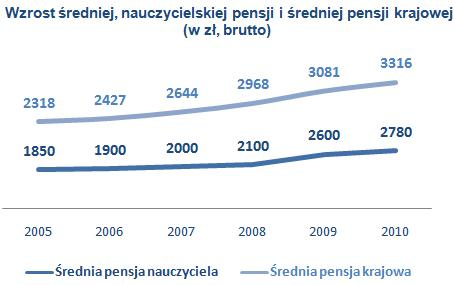
\includegraphics[width=200px]{images/pensja1} \end{center}

\end{frame}

\begin{frame}{Złe wykresy}

\begin{center}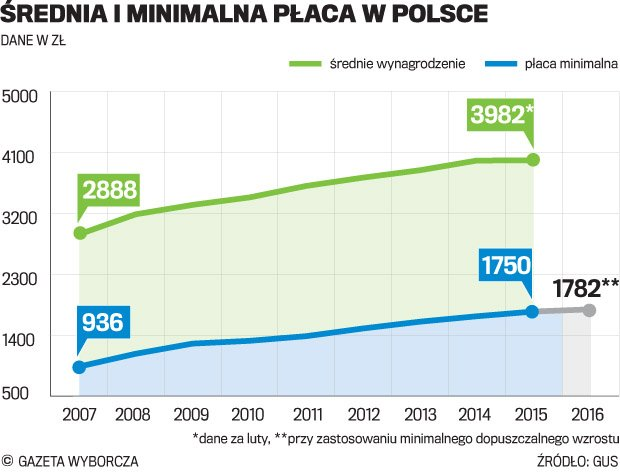
\includegraphics[width=200px]{images/pensja2} \end{center}

\end{frame}

\begin{frame}{Złe wykresy}

\begin{center}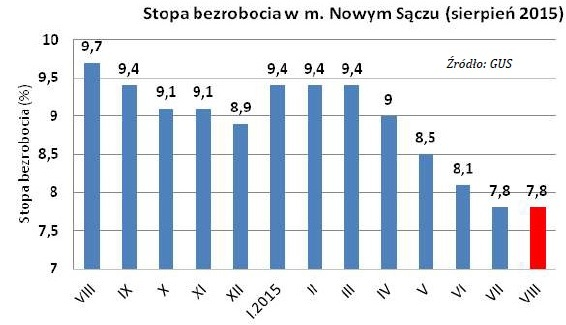
\includegraphics[width=200px]{images/bezrobocie01} \end{center}

\end{frame}

\begin{frame}{Złe wykresy}

\begin{center}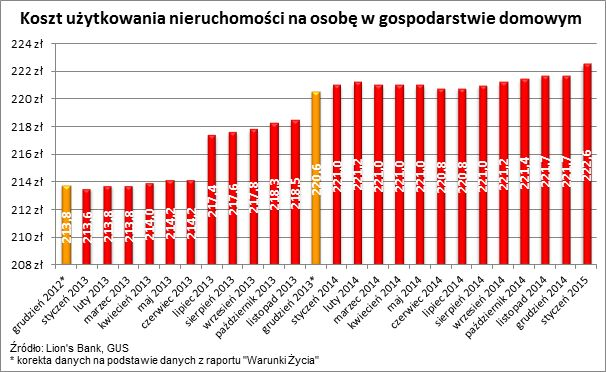
\includegraphics[width=200px]{images/koszt_utrzymania} \end{center}

\end{frame}

\begin{frame}{Złe wykresy}

\includegraphics{W4_files/figure-beamer/unnamed-chunk-8-1.pdf}

\end{frame}

\begin{frame}{Jakiego wykresu potrzebuję?}

Najpierw należy ustalić, co tak naprawdę chcemy zobaczyć na wykresie i
odpowiedzieć sobie na pytania:

\begin{itemize}
\tightlist
\item
  czy interesują nas konkretne wartości zmiennej, czy raczej ich
  rozkład?
\item
  czy dane zależą od czasu, a jeśli tak, to czy ta zależność nas
  interesuje?
\item
  czy danych jest dużo, czy niewiele?
\item
  czy dane są jedno-, czy wielowymiarowe?
\item
  i wiele innych\ldots{}
\end{itemize}

\end{frame}

\begin{frame}{Histogram}

\begin{itemize}
\tightlist
\item
  przedstawia rozkład naszej zmiennej
\item
  pozwala dostrzec pewne struktury w naszych danych
\item
  pomaga w wychwyceniu charakterystyki zmiennej
\item
  przestawia w zasadzie tylko jeden wymiar problemu
\item
  nie pokazuje zależności między zmiennymi
\item
  trzeba odpowiednio dobrać parametry, aby dostać rozsądną informację
\end{itemize}

\end{frame}

\begin{frame}{Histogram}

\includegraphics{W4_files/figure-beamer/unnamed-chunk-10-1.pdf}

\end{frame}

\begin{frame}{Histogram}

\includegraphics{W4_files/figure-beamer/unnamed-chunk-11-1.pdf}

\end{frame}

\begin{frame}{Histogram}

\includegraphics{W4_files/figure-beamer/unnamed-chunk-12-1.pdf}

\end{frame}

\begin{frame}{Histogram}

\includegraphics{W4_files/figure-beamer/unnamed-chunk-13-1.pdf}

\end{frame}

\begin{frame}{Histogram}

\includegraphics{W4_files/figure-beamer/unnamed-chunk-14-1.pdf}

\end{frame}

\begin{frame}{Wykres liniowy}

\begin{itemize}
\tightlist
\item
  przydatny jeśli wartość zmiennej zależy od czasu
\item
  nie pokazuje charakterystyki zbioru
\item
  czytelny tylko wtedy, kiedy nie ma gwałtownych i chaotycznych zmian w
  czasie
\end{itemize}

\end{frame}

\begin{frame}{Wykres liniowy}

\includegraphics{W4_files/figure-beamer/unnamed-chunk-15-1.pdf}

\end{frame}

\begin{frame}{Wykres liniowy}

\includegraphics{W4_files/figure-beamer/unnamed-chunk-16-1.pdf}

\end{frame}

\begin{frame}{Scatter plot}

\begin{itemize}
\tightlist
\item
  Wykres punktowy, przedstawia zależność pomiędzy zmiennymi
\item
  bardzo przydatny jeśli podejrzewamy, że zmienne są skorelowane i
  chcemy to sprawdzić
\item
  pozwala na oszacowanie charakterystyki zmiennej, zachowując informacje
  o korelacjach (w przeciwieństwie do histogramu)
\item
  pozwala na odnalezienie danych odstających
\end{itemize}

\end{frame}

\begin{frame}{Scatter plot}

\includegraphics{W4_files/figure-beamer/unnamed-chunk-17-1.pdf}

\end{frame}

\begin{frame}{Scatter plot}

\includegraphics{W4_files/figure-beamer/unnamed-chunk-18-1.pdf}

\end{frame}

\begin{frame}{Prezentacja danych - przykład}

\includegraphics{W4_files/figure-beamer/unnamed-chunk-19-1.pdf}

\end{frame}

\begin{frame}{Prezentacja danych - przykład}

\begin{itemize}
\tightlist
\item
  ze względu na obecność absurdalnie dużej wartości, odstającej od
  reszty, wykres jest nieczytelny
\item
  wartość ta jest najprawdopodobniej błędem (przebieg kilkuletniego
  samochodu większy niż 10 milionów kilometrów - nierealne)
\item
  na kolejnym slajdzie wyświetlimy krzywą przybliżającą średnie wartości
  przebiegu w zależności od roku produkcji samochodu
\end{itemize}

\end{frame}

\begin{frame}{Prezentacja danych - przykład}

\includegraphics{W4_files/figure-beamer/unnamed-chunk-20-1.pdf}

\end{frame}

\begin{frame}{Prezentacja danych}

\includegraphics{W4_files/figure-beamer/unnamed-chunk-21-1.pdf}

\end{frame}

\begin{frame}{Prezentacja danych}

\begin{itemize}
\tightlist
\item
  Po odflitrowaniu odstających i z pewnością błędnych wartości, wykres
  nadal jest dość mało czytelny
\item
  zbyt dużo punktów, zmienna ``x'' jest dyskretna
\item
  warto w takiej sytuacji zwizualizowac sobie zagregowane
  charakterystyki dla kolejnych wartości zmiennej ``x''
\end{itemize}

\end{frame}

\begin{frame}{Prezentacja danych}

\includegraphics{W4_files/figure-beamer/unnamed-chunk-22-1.pdf}

\end{frame}

\begin{frame}{Prezentacja danych}

\includegraphics{W4_files/figure-beamer/unnamed-chunk-23-1.pdf}

\end{frame}

\begin{frame}{Prezentacja danych}

\includegraphics{W4_files/figure-beamer/unnamed-chunk-24-1.pdf}

\end{frame}

\begin{frame}{Prezentacja danych}

\includegraphics{W4_files/figure-beamer/unnamed-chunk-25-1.pdf}

\end{frame}

\begin{frame}{Rozkłady - histogram}

\begin{itemize}
\tightlist
\item
  Losujemy po 100 próbek z rozkładu Gaussa i z rozkładu jednorodnego
\item
  Poniżej przedstawione są one na dwóch nieznacznie różniących się
  wykresach
\item
  Czy patrząc na drugi z wykresów bylibyśmy w stanie odgadnąć, z jakich
  rozkładów pochodzą nasze zmienne?
\end{itemize}

\end{frame}

\begin{frame}{Rozkłady - histogram}

\includegraphics{W4_files/figure-beamer/unnamed-chunk-26-1.pdf}

\end{frame}

\begin{frame}{Rozkłady - funkcja gęstości rozkładu}

\includegraphics{W4_files/figure-beamer/unnamed-chunk-27-1.pdf}

\end{frame}

\begin{frame}{Rozkłady - histogram}

\begin{itemize}
\tightlist
\item
  Kiedy próbek jest dużo (teraz 100000), jest znacznie łatwiej
\end{itemize}

\includegraphics{W4_files/figure-beamer/unnamed-chunk-28-1.pdf}

\end{frame}

\begin{frame}{Rozkłady - Q-Q plot}

\begin{itemize}
\tightlist
\item
  Często potrzebujemy sprawdzić (a przynajmniej upewnić się), z jakiego
  rozkładu pochodzi nasza zmienna
\item
  Jeśli mamy dużo próbek, rozkład można rozpoznać (oczywiście w
  przybliżeniu) z histogramu lub wykresu gęstości prawdopodobieństa
\item
  Jeśli jednak próbek jest mało, warto obejrzeć tzw. Q-Q plot pokazujący
  nam jak się mają obserwowane kwantyle naszego rozkładu do
  teoretycznych (z rozkładu, z którym porównujemy naszą próbę)
\end{itemize}

\end{frame}

\begin{frame}{Rozkłady - Q-Q plot}

\includegraphics{W4_files/figure-beamer/unnamed-chunk-29-1.pdf}

\end{frame}

\begin{frame}{Gdy próbek jest niewiele}

\includegraphics{W4_files/figure-beamer/unnamed-chunk-30-1.pdf}

\end{frame}

\begin{frame}{Gdy próbek jest niewiele}

\includegraphics{W4_files/figure-beamer/unnamed-chunk-31-1.pdf}

\end{frame}

\begin{frame}[fragile]{Mapy - Polska z Google Maps}

\begin{Shaded}
\begin{Highlighting}[]
\NormalTok{pol.map <-}\StringTok{ }\KeywordTok{get_map}\NormalTok{(}\DataTypeTok{location=}\KeywordTok{c}\NormalTok{(}\DataTypeTok{lon=}\DecValTok{20}\NormalTok{, }\DataTypeTok{lat=}\DecValTok{52}\NormalTok{),}
                   \DataTypeTok{zoom=}\DecValTok{6}\NormalTok{, }\DataTypeTok{maptype=}\StringTok{"hybrid"}\NormalTok{)}
\KeywordTok{ggmap}\NormalTok{(pol.map)}
\end{Highlighting}
\end{Shaded}

\includegraphics{W4_files/figure-beamer/unnamed-chunk-32-1.pdf}

\end{frame}

\begin{frame}{Mapy}

\begin{itemize}
\tightlist
\item
  przy tworzeniu mapy trzeba pamiętać, że oprócz wartości zmiennej
  potrzebujemy współrzędnych, aby odpowiednie wartości zmiennej nałożyć
  na odpowiednie miejsca na mapie
\item
  dane zwykle trzeba wcześniej skalibrować (w szczególności po względem
  geometrycznym)
\item
  dobrze dobrana skala jest tu bardzo istotna
\end{itemize}

\end{frame}

\begin{frame}{Mapy - południowa Polska nocą}

\includegraphics{W4_files/figure-beamer/unnamed-chunk-33-1.pdf}

\end{frame}

\begin{frame}{Mapy - Kraków i okolica nocą}

\includegraphics{W4_files/figure-beamer/unnamed-chunk-34-1.pdf}

\end{frame}

\begin{frame}{Ciekawe przykłady}

Histogram zapytań przedstawiony w postaci ``mapy ciepła''" (heatmap) -
za liczbę zliczeń odpowiada kolor słupka

\begin{center}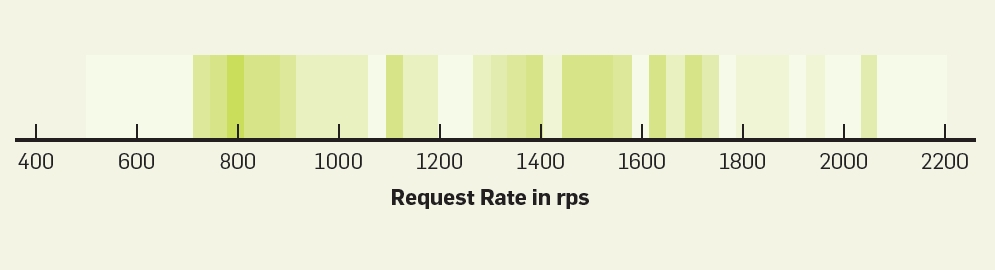
\includegraphics[width=300px]{images/rr_heatmap_hist} \end{center}

\end{frame}

\begin{frame}{Ciekawe przykłady}

Sekwencja czasowa histogramów (przedstawionych jako ``mapy ciepła'') -
oprócz ogólnej charakterystyki (rozkład bimodalny) widzimy też, jak
sytuacja zmieniała się w czasie - znacznie więcej informacji niż
``zwykły'' histogram

\begin{center}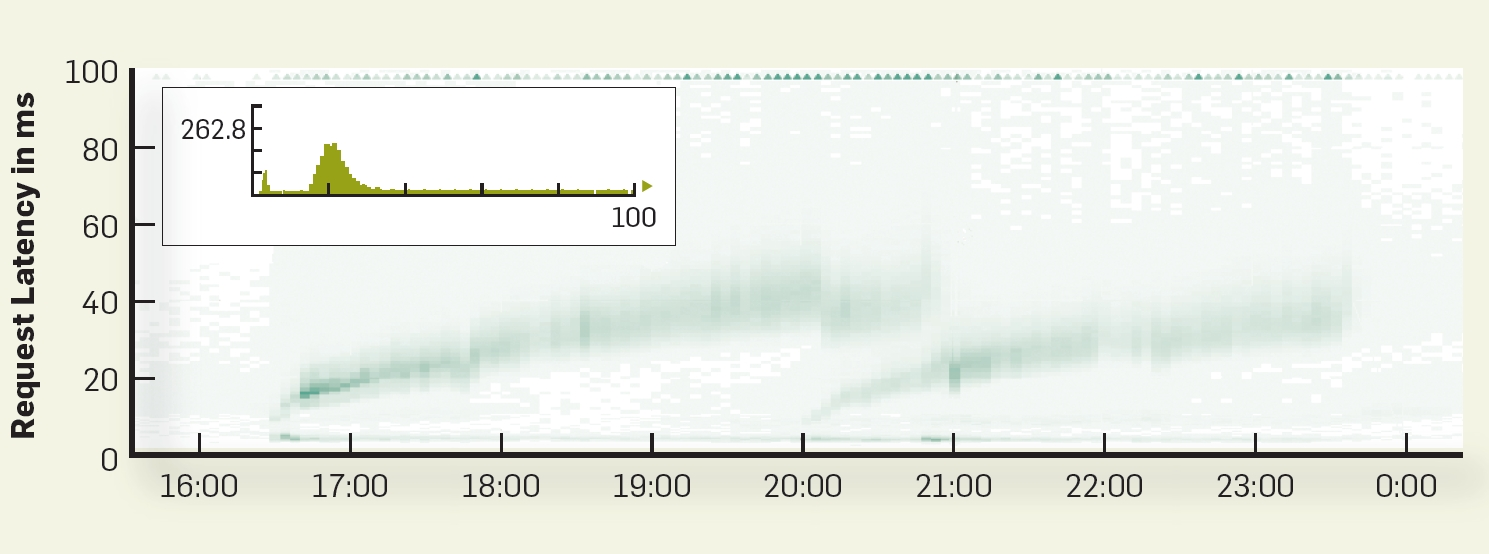
\includegraphics[width=300px]{images/r_latency} \end{center}

\end{frame}

\end{document}
